\documentclass[12pt]{article}
\usepackage[utf8]{inputenc}
\usepackage{graphicx}
\graphicspath{ {images/} }
\usepackage{multicol}
\usepackage{amsmath}
\setlength{\columnsep}{2cm}
\usepackage{float}
\usepackage[top=2cm, bottom=2cm, left=2cm, right=2cm]{geometry}

%\oddsidemargin=0pt % отступ от левого края
%\topmargin=-1.5cm % отступ от верхнего края

\usepackage[cp1251]{inputenc}
\usepackage[russian]{babel}
\begin{document}

\begin{titlepage}
	\centering
	{\scshape\LARGE Московский физико-технический институт \par}
	\vspace{3cm}
	{\huge\bfseries Вопрос по выбору \par}
	\vspace{1cm}
	{\huge\bfseries Исследование стационарного потока жидкости в трубе \par}
	\vspace{1cm}
	%{\Large\itshape John Birdwatch\par}
	\vfill
    
\begin{flushright}
	{\scshape\LARGE группа Б01-502}\par
	\vspace{0.3cm}
	{\scshape\LARGE Кокарев Константин} %\textsc{Brown}
\end{flushright}
	\vfill

\end{titlepage}

\section*{Цель работы}

\begin{itemize}
  \item Измерение скорости течения по методам Пито и Вентури.
  \item Сравнение результатов со скоростью, определённой по расходу воды.
\end{itemize}

\section*{Оборудование}

\begin{itemize}
  \item установка
  \item линейка
  \item секундомер
\end{itemize}

\section*{Теоретические справка}

В работе исследуется течение жидкости по трубе постоянного сечения.

Основной целью исследования потока жидкости или газа в трубе является определение скорости движения и расхода. Правильное определение расхода очень важно в прикладных задачах — в газо- и нефтепроводах, а также в водопроводе и при теплоснабжении.

Ввиду важности приложений было разработано много разных способов определения расхода и скорости потока жидкости или газа, но самые простые и в то же время точные основаны на измерении перепада давления, связанного либо с положением приемников — навстречу или вдоль потока (как в трубке Пито), либо вызванного специальным препятствием — типа сужения трубы (как в трубке Вентури) или установкой внутри трубы шайбы — кольца. 

Чтобы понять прицип работы различных расходомеров нужно используется уравнение Бернулли для несжимаемой жидкости:

\begin{equation}
p{}_1{} + \frac {\rho v{}_1{}^2}{2} + \rho gz{}_1{} = p{}_2{} + \frac {\rho v{}_2{}^2}{2} + \rho gz{}_2{}
\label{eq:bernuli}
\end{equation}


\section*{Расходомер Вентури}

\begin{figure}[H]
\centering
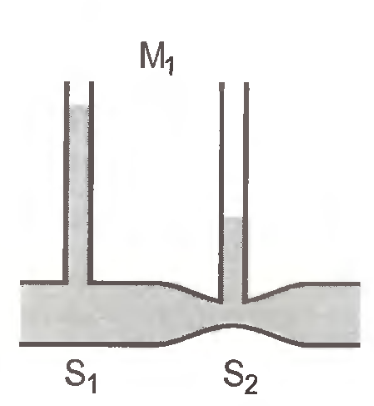
\includegraphics[width=0.5\textwidth]{venturi.png}
\caption{Расходомер Вентури}
\label{fig:venturi}
\end{figure}

Расходомер Вентури (рис.~1) представляет собой горизонтальную трубу с плавно меняющимся сечением. В широком (сечение \( S_1 \)) и узком (сечение \( S_2 \)) участках сделаны выводы к трубкам водяного манометра \( M_1 \). Высота поднятия воды в трубках манометра определяет давление в соответствующих сечениях.

В силу несжимаемости жидкости (\( v_1 S_1 = v_2 S_2 \)) и горизонтальности трубы (\( z_1 = z_2 \)) из уравнения Бернулли \eqref{eq:bernuli} получаем скорость потока в сечении \( S_1 \) через давления в сечениях \( S_1 \) и \( S_2 \):

\begin{equation}
v_1 = \sqrt{\frac{2(p_1 - p_2)}{\rho \left[ (S_1 / S_2)^2 - 1 \right]}}.
\label{eq:venturi}
\end{equation}

\section*{Расходомер Пито}

\begin{figure}[H]
\centering
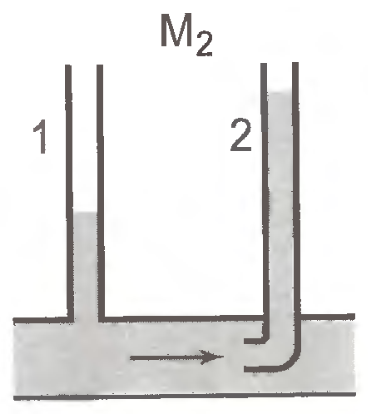
\includegraphics[width=0.5\textwidth]{pito.png}
\caption{Расходомер Пито}
\label{fig:pito}
\end{figure}

Расходомер Пито изображен на рис.~2. С исследуемой трубой \( T \) соединены две трубки водяного манометра \( M_2 \). Одна из них (1) подведена к стенке трубы \( T \), а другая (2) изогнута и направлена открытым концом навстречу потоку. Перед отверстием трубы 2 жидкость неподвижна, \( v_2 = 0 \). 

Пусть давления, измеренные манометрическими трубками 1 и 2, равны \( p_1 \) и \( p_2 \). Уравнение Бернулли дает:

\[
p_1 + \frac{\rho v_1^2}{2} = p_2,
\]

откуда

\begin{equation}
v_1 = \sqrt{\frac{2(p_2 - p_1)}{\rho}}.
\label{eq:pito}
\end{equation}

Уравнение (\ref{eq:pito}) позволяет связать скорость жидкости с разностью высот в трубках манометра \( M_2 \).

С помощью трубки Пито измеряется локальная скорость потока в месте расположения трубки, при помощи него можно измерить профиль скорости в трубе (измерять в разных местах), а в методе Вентури измеряется лишь средняя скорость по сечению трубы. Если нужно измерить только расход, то можно применить метод Вентури, в котором расход вычисляется по некоторой усредненной по сечению трубы скорости. Когда требуется определить скорость потока, то нужно использовать трубку Пито. Чаще такая необходимость возникает не при измерениях в трубе, а при исследовании внешнего потока. Трубка Пито применяется в самом широком диапазоне скоростей — от измерений медленных движений в вязком пограничном слое и до измерений сверхзвуковых скоростей на самолетах.

\begin{figure}[H]
\centering

\includegraphics[width=0.5\textwidth]{turb.png}
\caption{профили потока при ламинарном и турбулентном течении}
\label{fig:turb}
\end{figure}

При использовании трубопроводов всегда важно знать объем или массу среды, протекающей за единицу времени. Измерения осложняются влиянием вязкости, из-за которой и жидкость, и газ «прилипают» к стенке, около которой скорость равна нулю. Поэтому в трубе скорость всегда изменяется вдоль радиуса, всегда увеличивается в той или иной степени по направлению от стенки к оси трубы. Если используется установившееся движение при относительно малых числах Рейнольдса, то применима формула Пуазейля, и в таком случае достаточно измерить скорость в одной точке, например, на оси трубы. Объёмный расход определяется законом Пуазейля:

\begin{equation}
Q = \frac{\pi R^4 \Delta p}{8 \eta L}
\label{eq:poiseuille}
\end{equation}

В других случаях для правильного определения расхода требуется проинтегрировать скорость по площади, для чего нужно произвести измерения в нескольких точках. Например, рекомендуется использовать 20 трубок Пито, размещенных на разных расстояниях от оси трубы по двум взаимно перпендикулярным направлениям.

\section*{Ультразвуковой расходомер}

\begin{figure}[H]
\centering
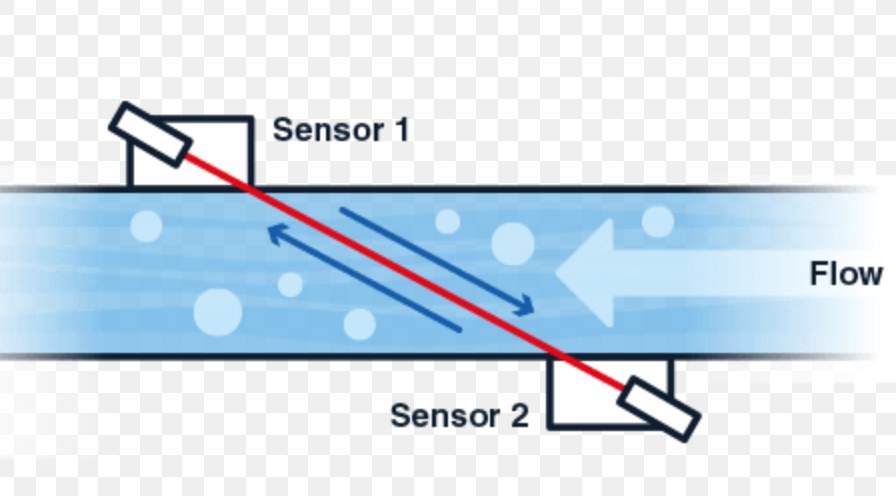
\includegraphics[width=0.8\textwidth]{ultra.png}
\caption{Ультразвуковой расходомер}
\label{fig:ultra}
\end{figure}

К физическим методам определения расхода жидкости или газа относится ультразвуковой расходомер. Этот способ основан на том, что в движущейся среде звук, который распространяется относительно среды с постоянной скоростью, движется вместе с нею, и поэтому в направлении движения жидкости или газа скорость звука больше, а против — меньше, чем в покоящейся среде. Излучатель и приемник ультразвука устанавливаются на противоположных стенках канала или трубы с определенным сдвигом вдоль оси, так что ультразвук распространяется под некоторым углом к направлению скорости потока. Поэтому скорость в направлении движения больше, а в противоположном направлении меньше, чем в неподвижной среде. Разница между ними с учетом угла определяет скорость потока. Преимущество ультразвукового расходомера в том, что его работа не зависит от вязкости среды. Однако в таких условиях измеряется некоторая средняя скорость на пути звукового луча, поэтому для точных измерений прибор нуждается в градуировке. При этом градуировка будет зависеть в том числе и от числа Рейнольдса, так как от него зависит профиль скорости среды.

\section*{Турбинный расходомер}

\begin{figure}[H]
\centering
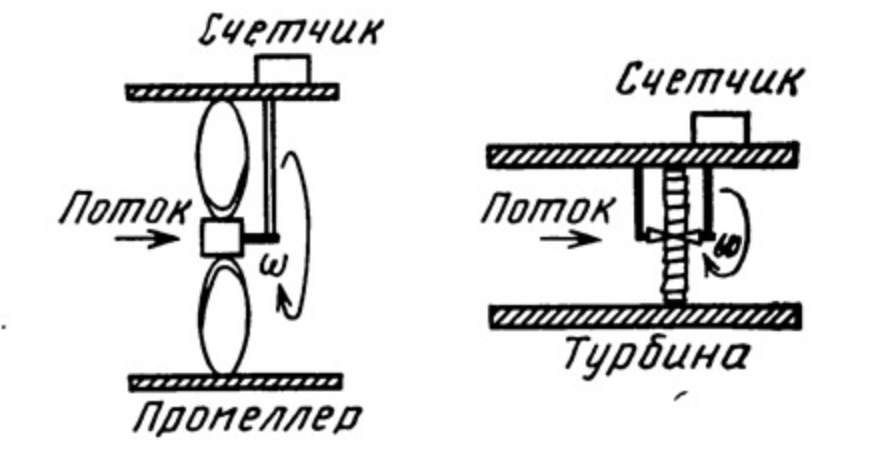
\includegraphics[width=0.8\textwidth]{turbina.png}
\caption{Турбинный расходомер}
\label{fig:setup}
\end{figure}

Отметим также турбинный расходомер, в котором расход пропорционален числу оборотов турбинки. Однако его показания сильно зависят от вязкости среды.

\section*{Экспериментальная установка}

\begin{figure}[H]
\centering
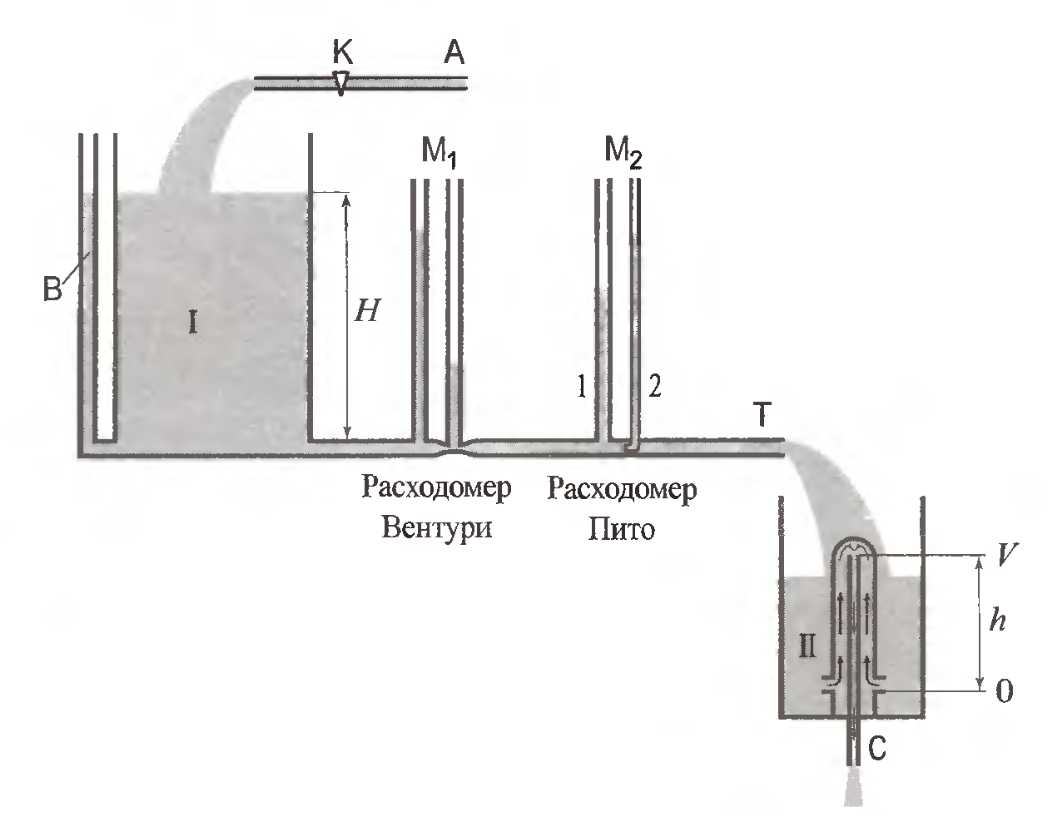
\includegraphics[width=0.8\textwidth]{setup.png}
\caption{Схема установки для исследования стационарного потока жидкости в трубе}
\label{fig:setup}
\end{figure}

Схема установки, служащей для исследования течения воды в трубе, изображена на рис.~6. Вода поступает в трубу \( T \) из цилиндрического резервуара I, снабженного водомерной трубкой \( B \) из стекла. Наполнение резервуара производится из водопровода по трубе \( A \) и регулируется краном \( K \). Выливающаяся из трубы \( T \) вода попадает в приемный резервуар II, в дно которого вмонтирован сифон \( C \).

Сифон предохраняет резервуар от переполнения, автоматически выливая из него воду, как только ее уровень достигнет высоты \( h \). Труба \( T \) снабжена расходомерами Вентури и Пито.

Скорость течения, усредненную по сечению трубы, можно определить по расходу, который находится по измеренному времени наполнения резервуара II, объем которого задан. С другой стороны, скорость может быть рассчитана по показаниям манометров с помощью формул (\ref{eq:venturi}) и (\ref{eq:pito}). Сопоставление этих скоростей со скоростью, определенной по расходу, позволяет сделать вывод о применимости уравнения Бернулли, роли вязкости, которая, в частности, приводит к изменению скорости поперек потока.

До сих пор предполагалось, что жидкость идеальная и потерь на трение при ее движении в трубе \( T \) не происходит. Для количественной оценки роли вязкости необходимо проделать следующий эксперимент. Установив уровень жидкости в резервуаре I на определенной высоте \( z_1 \), измерить скорость течения жидкости по трубе \( T \) с помощью приемного резервуара II (в силу несжимаемости жидкости ее скорость на входе в трубу \( T \) и на выходе из нее одинакова). По измеренному значению скорости по формуле Торричелли рассчитывать ту высоту \( z_2 \), при которой жидкость вытекала бы с этой же скоростью в отсутствие вязкости. Формула Торричелли для истечения струи жидкости из отверстия:

\begin{center}
$ v=\sqrt{2gz_2} $
\end{center}

Разность \( z_1 - z_2 \) характеризует потери на внутреннее трение в жидкости, причем можно считать, что эти потери происходят только в трубе \( T \), так как скорость жидкости в резервуаре I существенно меньше.

Влияние вязкости изменяет показания манометра Вентури \( \Delta h \) на величину, которую можно оценить, умножив разность \( z_1 - z_2 \) на отношение расстояния между входами манометра \( \Delta l \) ко всей длине трубы \( L \). При условии

\[
\Delta h \gg (z_1 - z_2) \frac{\Delta l}{L}
\]

неидеальностью жидкости в пределах манометра можно пренебречь. В противном случае (\( \Delta h \) сравнимо с \( (z_1 - z_2) \frac{\Delta l}{L} \)) в уравнении (\ref{eq:venturi}) из \( p_1 - p_2 \) необходимо вычесть \( \Delta z \frac{\Delta l}{L} \rho g \).

Все сказанное относится и к расходомеру Пито. Кроме этого, для трубки Пито следует сделать оценку поправки к его показаниям, вызванную конечностью размеров вставленной в поток частью изогнутой трубки 2.

При измерениях очень важно обеспечить стационарность течения жидкости. Это достигается тем, что уровень воды в резервуаре I при каждом измерении с помощью крана \( K \) должен поддерживаться на одной и той же высоте \( H \). 

\section*{Ход работы}

\begin{enumerate}
\item Проверим исправность установки: после пуска воды закроем конец трубы пробкой. Уровни воды в манометрах расходомеров совпали.

\item Параметры установки
\begin{itemize}
    \item Длина трубы: $L = 65,20 \pm 0,05$ см
    \item Длина основания:  $a = 19,50 \pm 0,05$ см
    \item Ширина основания: $b = 19,50 \pm 0,05$ см
    \item Высота до сифона: $c = 31,00 \pm 0,05$ см
    \item Диаметр трубки: $d = 1,00 \pm 0,05$ см
    \item Радиус трубки:  $R = 0,50 \pm 0,05$ см
    \item Диаметр узкой части Вентури: $d_{\text{в}} = 0,60 \pm 0,05$ см
    \item Радиус трубки Пито: $r = 0,02 \pm 0,05$ см
    \item Расстояние между трубками Вентури: $\Delta l_{\text{в}} = 2,50 \pm 0,05$ см
    \item Расстояние между трубками Пито: $\Delta l_{\text{п}} = 2,00 \pm 0,05$ см
\end{itemize}

\item Проведем 8 измерений для различных высот столба воды, и занесем полученные данные в таблицу

\begin{table}[H]
\centering
\caption{Результаты измерений}
\label{tab:results}
\begin{tabular}{|c|c|c|c|c|c|c|c|c|}
\hline
$H$, см              & 5      & 10     & 20      & 25     & 30     & 40     & 50\\
\hline
$t$, с               & 890.14 & 669.62 &  620.13 & 409.25 & 365.86 & 310.12 & 270.54\\
\hline
$\Delta h_{\text{в}}$, мм   & 14     & 19     & 43      & 50     & 59     & 83     & 108\\
\hline
$\Delta h_{\text{п}}$, мм   & 2      & 5      & 8       & 11     & 12     & 17     & 20 \\
\hline
$v_p$, м/с           & 0.169  & 0.226  & 0.244   & 0.370  & 0.414  & 0.489  & 0.560\\
\hline
$v_t$, м/с           & 1      & 1,4    & 1,9     & 2,21   & 2,42   & 2,8    & 3,13\\
\hline
$\sigma_{v_p}$, м/с  & 0.005  & 0.006  & 0.006   & 0.007  & 0.008  & 0.01   & 0.01\\
\hline
Re                   & 845    & 1130   & 1220    & 1850   & 2070   & 2445   & 2800\\
\hline
\end{tabular}
\end{table}

\item При этом для расчета погрешности воспользуемся следующей формулой:

\[
\varepsilon_{v_p} = \sqrt{\left(\frac{\sigma_a}{a}\right)^2 + \left(\frac{\sigma_b}{b}\right)^2 + \left(\frac{\sigma_c}{c}\right)^2 + \left(\frac{\sigma_t}{t}\right)^2 + 4 \left(\frac{\sigma_{d}}{d}\right)^2}
\]

Абсолютную погрешность секундомера считаем равной 0,5 c

\item Значения, вычисленные по формуле Торричели, превосходят значения, полученные эксперементально, введу явления вязкости и трения, которое не учитывается в формуле Торричелли.
Различие видно на рисунке 7, на которой представленна теоретическая зависимость по формуле Торричели и аппроксимируюшая прямая по эксперементальным данным.

\begin{figure}[H]
\centering
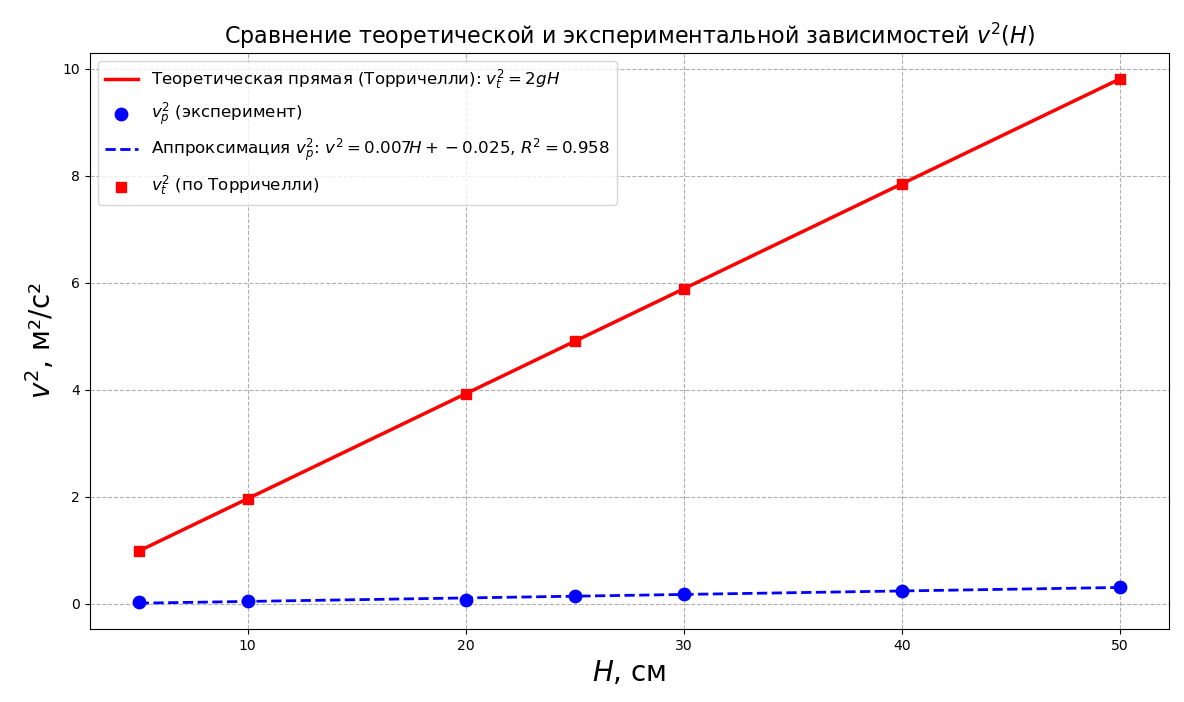
\includegraphics[width=0.8\textwidth]{Tor_g.png}
\caption{Сравнение теоретических и экспеременатльных данных}
\label{fig:setup}
\end{figure}

Наблюдаем несовпадение эксперементального и теоретического значений. Возможные причины:
\begin{itemize}
  \item Не учитывалась вязкость воды при расчёте предполагаемой высоты столба
  \item Турбулентный характер движения воды в резервуаре I при его заполнении
  \item То есть, неидеальность жидкости
\end{itemize}

\item По формулам для расходомеров Вентури и Пито вычислим скорость течения. Сначала вычисления проведём без учёта потерь, затем с ними. Результаты занесём в таблицу 2.

\begin{table}[H]
\centering
\caption{Результаты вычислений}
\label{tab:results}
\begin{tabular}{|c|c|c|c|c|c|c|c|c|}
\hline
$H$, см                       & 5      & 10     & 20      & 25     & 30     & 40     & 50\\
\hline
$v_{\text{В}}$, м/с           & 0.202  & 0.235  & 0.354   & 0.381  & 0.415  & 0.492  & 0.561\\
\hline
$v_{\text{П}}$, м/с           & 0.197  & 0.313  & 0.395   & 0.464   & 0.484 & 0.577  & 0.626\\
\hline
$\sigma_{v_{\text{В}}}$, м/с  & 0.008  & 0.008  & 0.01   & 0.011  & 0.012  & 0.013   & 0.013\\
\hline
$\sigma_{v_{\text{П}}}$, м/с  & 0.031  & 0.022  & 0.018   & 0.017  & 0.015  & 0.012   & 0.011\\
\hline
$v_{\text{В-попр}}$, м/с      & 0.188  & 0.211  & 0.322   & 0.345  & 0.374  & 0.446  & 0.511\\
\hline
$v_{\text{П-попр}}$, м/с      & 0,161  & 0,256  & 0,323   & 0,380  & 0.396  & 0,473 & 0.513\\
\hline
\end{tabular}
\end{table}

\begin{figure}[H]
\centering
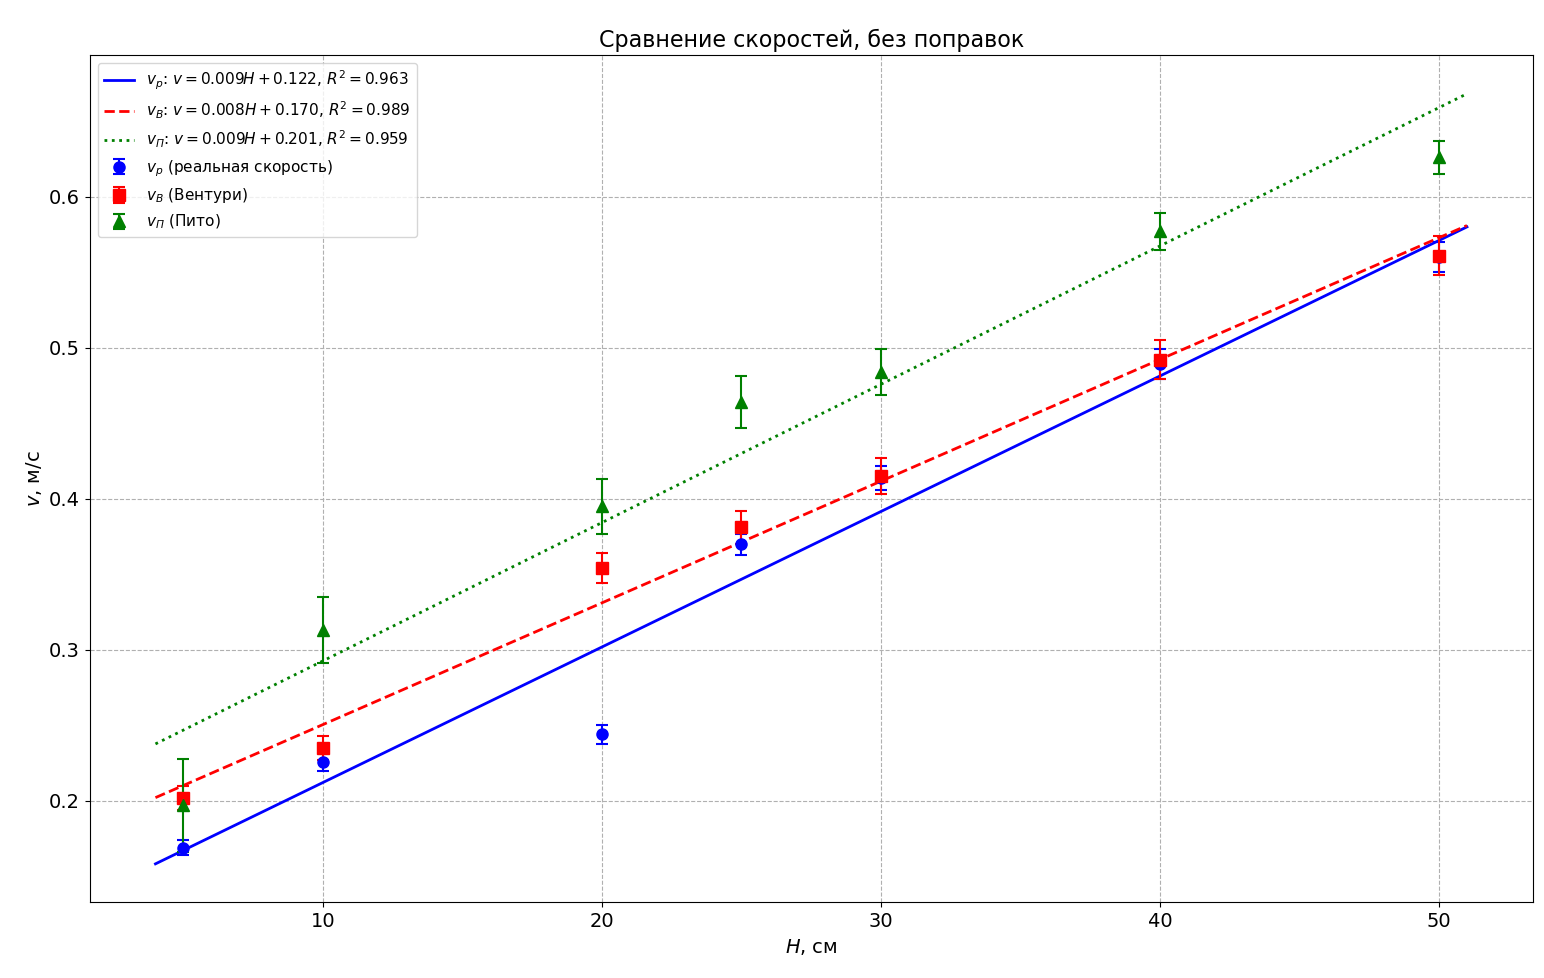
\includegraphics[width=0.8\textwidth]{Speed_no_pop.png}
\caption{Сравнение скоростей полученных в разных расходомерах}
\label{fig:setup}
\end{figure}

Преобразуем формулы. Для трубки Пито(из формулы (3)):
\[
v_{\Pi} = \sqrt{2g \Delta h_{\Pi}}.
\]

Для расчёта погрешности \( v_{\Pi} \) имеем:
\[
\sigma^2_{v_{\Pi}} = \left( \frac{\partial v_{\Pi}}{\partial \Delta h} \right)^2 \cdot \sigma^2_{\Delta h} 
= \frac{g}{2 \Delta h} \cdot \sigma^2_{\Delta h}.
\]

Для трубки Вентури (из формулы (2)):
\[
v_B = \sqrt{\frac{2g \Delta h_{\text{в}}}{\left( \frac{S_1}{S_2} \right)^2 - 1}},
\]

где 
\[
S_1 = \pi \cdot \left( \frac{d}{9} \right)^2, \quad 
S_2 = \pi \cdot \left( \frac{d_{\text{в}}}{9} \right)^2.
\]

Расчёта погрешности \( v_B \):

\[
\varepsilon_{S_1} = \sqrt{4 \left( \frac{\sigma_{d}}{d} \right)^2 + 4 \left( \frac{\sigma_{d_{\text{в}}}}{d_{\text{в}}} \right)^2},
\]

\[
\sigma_{v_B}^2 = \left( \frac{\partial v_B}{\partial \Delta h} \right)^2 \cdot \sigma_{v_B}^2 + \left( \frac{\partial v_B}{\partial \left( \frac{S_1}{S_2} \right)} \right)^2 \cdot \sigma_{v_B}^2.
\]

С учётом поправки на вязкость для \( v_B \) имеем:

\[
v_B = \sqrt{\frac{2g\left(\Delta h - \Delta z \frac{\Delta l}{L}\right)}{\left( \frac{S_1}{S_2} \right)^2 - 1}}.
\]

Для расходомера Пито проведём следующую оценку\\
Скорость жидкости в центре трубы по формуле Пуазейля:
\begin{center}
$v_0 =\frac{1}{4\nu}\frac{\triangle P}{L}(R^2)$
\end{center}
Скорость жидкости у края трубки расходомера Пито:\\
\begin{center}
$v(r) =\frac{1}{4\nu}\frac{\triangle P}{L}(R^2-r^2)$
\end{center}
Средняя скорость в трубке Пито:\\
\begin{center}
$v_m =\frac{1}{4\nu}\frac{\triangle P}{L}(R^2-\frac{r^2}{2})$
\end{center}
Тогда\\
\begin{center}
$\frac{1}{4\nu}\frac{\triangle P}{L} =\frac{v_0}{R^2}$
\end{center}
Окончательно средняя скорость воды в трубе:\\
\begin{center}
$v_m =\frac{v_0({R^2-\frac{r^2}{2}}) }{R^2}$
\end{center}

\item Изобразим на рисунке 9, скорости воды с учетом поправок для каждого из расходомера.

\begin{figure}[H]
\centering
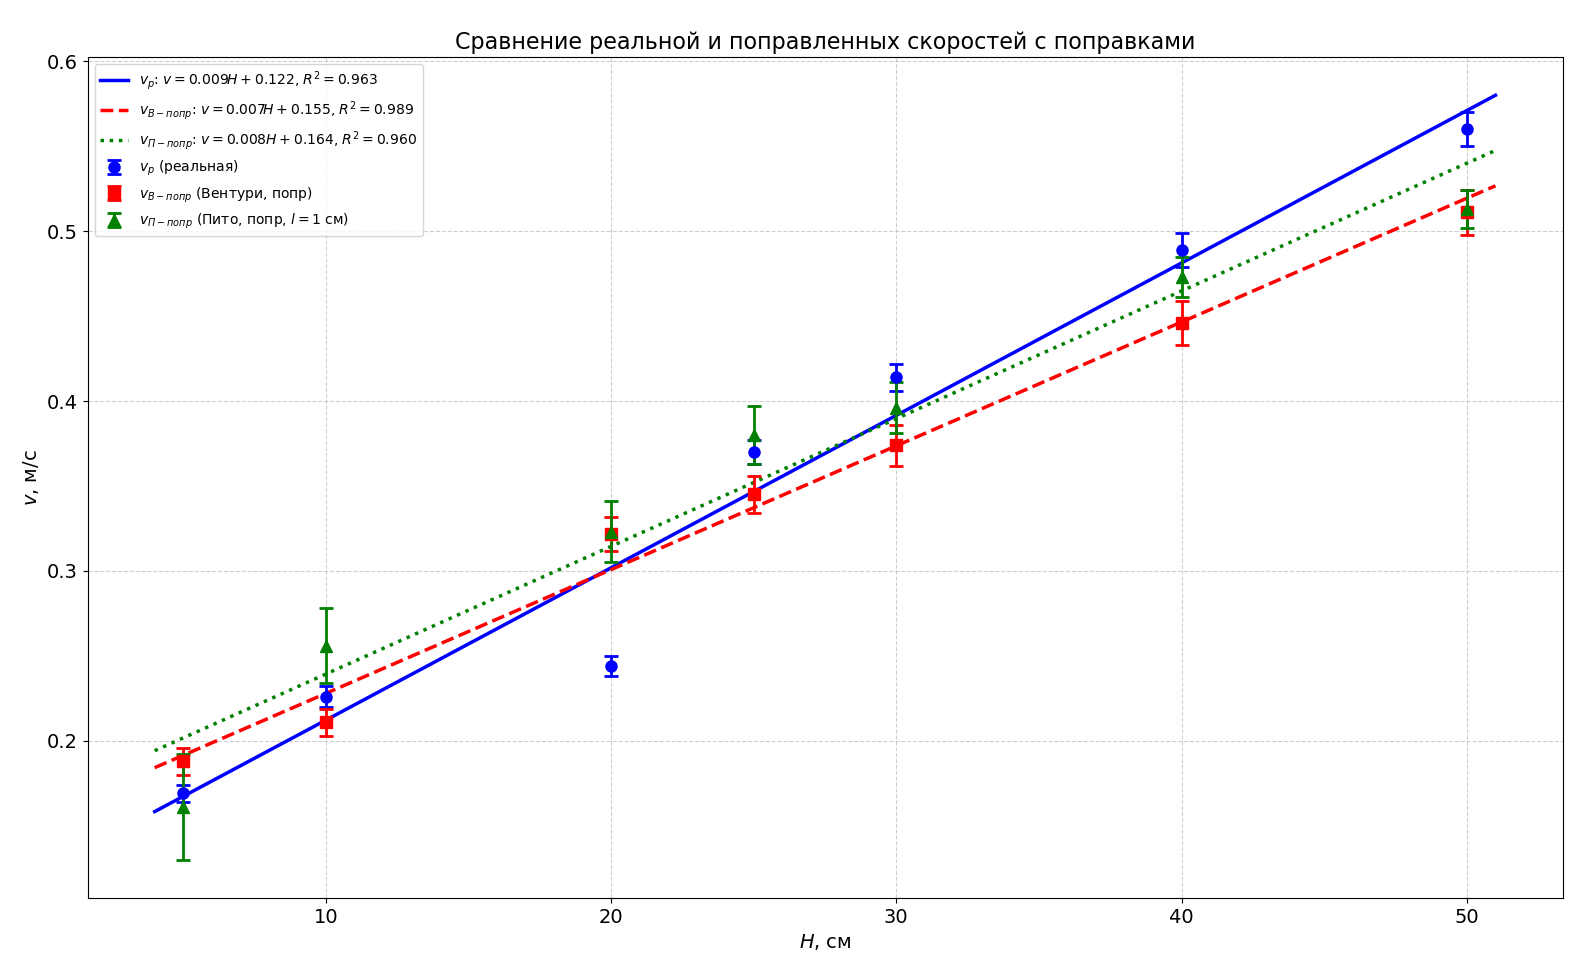
\includegraphics[width=0.8\textwidth]{Speed_pop.png}
\caption{Сравнение скоростей полученных в разных расходомерах с поправками}
\label{fig:setup}
\end{figure}

Видим, что с учетом поправко графики стали примерно равными\\

\item Построим график зависимости скорости течения по расходу от высоты столба воды рисунок 10

\begin{figure}[H]
\centering
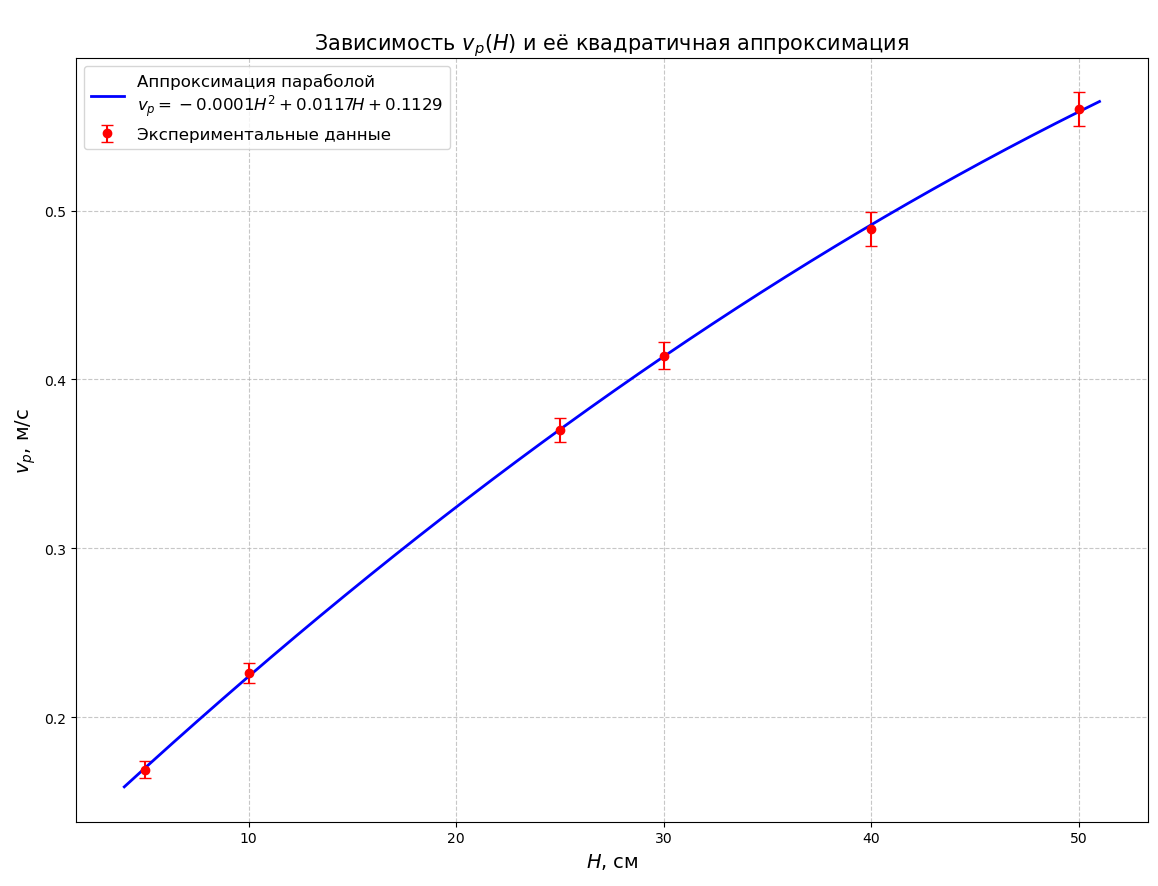
\includegraphics[width=0.8\textwidth]{V_p(H).png}
\caption{Зависимость скорости от высоты}
\label{fig:setup}
\end{figure}

По графику определим участки ламинарного и турбулентного течений. Сравним данный полученные из графика с  числами Рейнольдса подсчитанные для каждой скорости. 
Теоретическая скорость, когда течение станет турбулентным: $v = 0.355$м/с
Стоит отметить, что при достижении достаточно больших скоростей в трубе наблюдалось образование пузырьков жидкости, что также является признаком турбулентного течения жидкости

\end{enumerate}

\section*{Вывод}

В ходе работы было исследовано течение жидкости в цилиндрической трубе, изучен принцип работы расходомеров Вентури и Пито, исследованы ламинарный и стационарный режимы течения жидкости. 
\begin{itemize}
  \item Выяснено, что использование уравнения Торричелли для расчёта столба жидкости по скорости её течения неуместна по причине того, что рассматривается реальная, а не идеальная жидкость. Учитывая явно турбулентный характер движения жидкости в резервуаре при его заполнении, использование любых формул для ламинарного истечения из него неуместно
  \item Исследованы расходомеры Пито и Вентури, определены поправки для более точного расчёта скорости воды по их показаниям. Вязкость и трение об стенки играет огромную роль. Выяснилось, что наиболее точным является расходомер Вентури. Расходомер Пито показывает повышенное значение скорости, так как его трубка расположена в центре потока (пуазейлевкий профиль скоростей в реальной жидкости). Для более точных измерений с помощью расходомера Пито необходимо использовать несколько расходомеров, расположив их на разных расстояниях он центра трубы и усреднив полученные значения.
  \item По графику зависимости скорости течения от высоты столба жидкости определены участки ламинарного и турбулентного течения воды, найдена точка, в которой предположительно течение меняет характер с ламинарного на турбулентное;
  \item Поправка на радиус трубки Пито рассчитана в предположении параболического профиля скоростей (закон Пуазейля). Однако из-за того, что длина установления потока 
\[
L_{\text{уст}} \approx 0.05 \cdot Re \cdot D
\]
для воды при \(Re \sim 2000\) и \(D = 1\) см составляет \(L_{\text{уст}} \approx 1\) м, что превышает длину трубы \(L = 0.65\) м, профиль скоростей в месте установки трубки Пито не является полностью параболическим. Поэтому использование данной поправки вносит дополнительную систематическую погрешность, что отражено на графиках. Полученные значения \(v_{\text{П-попр}}\) следует рассматривать как оценочные.
\end{itemize}

\end{document}
